\documentclass[letterpaper,12pt,oneside]{article}
\usepackage[top=1in, left=1.25in, right=1.25in, bottom=1in]{geometry}

\usepackage[T1]{fontenc}
\usepackage[utf8]{inputenc}
\usepackage[english]{babel}
\usepackage{caption, subcaption} %figuras
\usepackage{graphicx}
\usepackage{array}
\usepackage{amsmath} 
\usepackage{amssymb} 
\usepackage{tikz}
\usepackage{imakeidx}
\usepackage{biblatex}
\addbibresource{bib/protocolo.bib}

\graphicspath{{./figs/}}
\usepackage{setspace}
%\usepackage[round]{natbib}

\begin{document}
%\frontmatter
\begin{titlepage}
		\setlength{\parindent}{0pt} \setlength{\parskip}{0pt}
	
		\begin{center}
			\vfill 
			
			\begin{minipage}{\textwidth}
				
				\newcolumntype{V}{>{\centering\arraybackslash} m{.17\textwidth} }
				\newcolumntype{C}{>{\centering\arraybackslash} m{.56\textwidth} }
				
				\begin{center}
					
\includegraphics[width=4.5cm]{UNAM_LOGO2.png}	
				\end{center} 	
				\begin{center}
					\Huge\textbf{Universidad Nacional Autónoma de México}
				\end{center} 
				
			\end{minipage}
				
			\vfill
			
			\begin{minipage}{0.7\textwidth}
				\begin{center}
					\large Ingeniería en Computación
				\end{center}
			\end{minipage}
			% 
			\begin{center}
				%\medskip \rule{.9\textwidth}{2pt}
				\vfill
				\large Compilers
				%{\Large \bfseries  \title   }
				
				%\medskip \rule{.9\textwidth}{2pt}
			\end{center}
			
			\begin{center}
				\vspace*{1cm}
				{\huge Parser and SDT}\\
				\vspace*{1cm}
				
				%PRESENTA:\\ \medskip
				\begin{center}
					STUDENTS: \\
					\large 321184995\\
					\large 321331656\\
					\large 321058526\\
					\large 424138220\\
					\large 320560154
				\end{center}
				
				\bigskip
				
				Group: \\
				\#05\\
				%Coadvisors
				Semester: \\
				2026-II
			\end{center}
			
			\vfill
			
			\begin{center}
				{México, CDMX. April 30th, 2025}\\
			\end{center}
			\cleardoublepage
		\end{center}
	\end{titlepage}
 
\tableofcontents
\clearpage
    
%\mainmatter

\section{Introduction} %
	
	In the construction of a compiler, one of the most critical phases after lexical analysis is syntax analysis (parsing) and semantic analysis. The lexical analyzer converts a source code string into a stream of tokens, but it does not verify whether the sequence of tokens follows the grammatical structure of the programming language, nor does it enforce semantic rules such as type consistency or variable declaration before use.
	
	\vspace{8pt}
	
	The specific problem addressed in this work is the implementation of a syntax and semantic analyzer that:
	
	\begin{itemize}
		\item Receives a sequence of tokens from a lexical analyzer.
		\item Determines whether the token sequence conforms to a context-free grammar defining the source language.
		\item Performs syntax-directed translation to verify semantic rules and build auxiliary structures such as the symbol table and the abstract syntax tree.
	\end{itemize}
	
	The input language is limited but realistic: it supports variable declarations (e.g., \textit{float y}, \textit{int x}), arithmetic expressions with parentheses and operators and assignment statements terminated by a semicolon. The compiler stops after semantic validation.
	
	\vspace{8pt}
	
	Understanding how a compiler verifies the correctness of a program before executing it is fundamental in computer engineering. While lexers are relatively simple, parsing and semantic analysis pose significant challenges: handling recursion, precedence, associativity, and context‑sensitive constraints.
	
	\vspace{8pt}
	
	Implementing a bottom‑up LALR parser from first principles — without relying on parser generators like Yacc or ANTLR — provides deep insight into:
	
	\begin{itemize}
		\item How LR automata work (states, goto, action tables).
		\item How shift‑reduce parsing uses explicit stacks to simulate a deterministic pushdown automaton.
		\item How syntax‑directed translation can be embedded into the parsing process to perform semantic checks and construct intermediate representations.
	\end{itemize}
	
	Furthermore, this project demonstrates the synergy between theoretical concepts and practical software engineering.
	
	\noindent\subsection*{General Objective:}
	
	Develop a functional syntax and semantic analyzer that, given a token stream from a lexical analyzer, verifies grammatical correctness, executes syntax‑directed translation rules, and produces a symbol table and an abstract syntax tree.
	
	\noindent\subsection*{Specific Objectives:}
	
	\begin{enumerate}
		\item Define a context‑free grammar that describes the subset of the source language (declarations, expressions, assignments).
		\item Construct an LALR parsing table from the grammar using closure, goto, first sets, and item set construction.
		\item Implement a shift‑reduce parser using two stacks (states and symbols) that simulates an LR automaton.
		\item Augment the grammar with SDT rules to:
			\begin{itemize}
				\item Check that variables are declared before use.
				\item Verify type compatibility in assignments and expressions.
				\item Build a symbol table.
				\item Build an AST representing the structure of each statement.
			\end{itemize}
		\item Provide clear output messages indicating:
			\begin{itemize}
				\item Parsing success/failure.
				\item SDT verification success/failure.
				\item Symbol table and a graphic AST.
			\end{itemize}
	\end{enumerate}
	
	
\section{Theoretical Framework}
	
	This section presents the compiler concepts applied in our implementation, directly referencing our code structure.
	
	\subsection{Lexical Analysis}
	
	The lexer converts source code into a stream of tokens. Our lexer uses \textbf{regular expressions} defined in the token list. Each regex pattern is matched sequentially against the input string.
	
	\textbf{Key concepts:}
	\begin{itemize}
		\item \textbf{Tokens}: pairs of (type, value) e.g., \texttt{('keyword', 'float')}, \texttt{('identifier', 'y')}
		\item \textbf{Pattern matching}: each pattern is tried until a match is found
		\item \textbf{Whitespace and comments}: patterns with token type \texttt{None} are ignored
		\item The lexer returns an error if an invalid character is found
	\end{itemize}
	
	In our code, the \texttt{tokenize()} function scans line by line, column by column, building the token list.
	
	\subsection{Grammar Definition}
	
	A \textbf{CFG} defines the syntactic structure of our language. We use the following grammar:
	
	\[
	\begin{array}{lcl}
		S' & \rightarrow & S \\
		S & \rightarrow & D \; ; \\
		D & \rightarrow & \text{TYPE} \; \text{ID} \; = \; E \\
		E & \rightarrow & E \; + \; T \;\;|\;\; T \\
		T & \rightarrow & T \; * \; F \;\;|\;\; F \\
		F & \rightarrow & ( \; E \; ) \;\;|\;\; \text{ID} \;\;|\;\; \text{CONST}
	\end{array}
	\]
	
	\noindent\textbf{Terminals} (tokens from lexer): \{\texttt{TYPE}, \texttt{ID}, \texttt{CONST}, \texttt{=}, \texttt{;}, \texttt{+}, \texttt{*}, \texttt{(}, \texttt{)}, \texttt{\$}\}\\
	\textbf{Non-terminals}: \{\texttt{S'}, \texttt{S}, \texttt{D}, \texttt{E}, \texttt{T}, \texttt{F}\}
	
	\subsection{LR(1) Items and Closure}
	
	An \textbf{LR(1) item} is a production with a dot ($\bullet$) indicating how much we have parsed, plus a lookahead terminal. Example:
	
	\[
	E \rightarrow E \; \bullet \; + \; T \quad , \quad \text{lookahead} = \{ \$, +, ) \}
	\]
	
	The \textbf{closure operation} (implemented in \texttt{cierre\_lr1()}) expands a set of items:
	\begin{enumerate}
		\item Start with the initial set of items
		\item If the dot is before a non-terminal $B$, add all productions of $B$ with the dot at the beginning
		\item Calculate lookaheads using FIRST sets
		\item Repeat until no new items can be added
	\end{enumerate}
	
	\subsection{FIRST Sets}
	
	FIRST($\alpha$) is the set of terminals that can begin strings derived from $\alpha$.
	
	\textbf{Calculation algorithm in our code}:
	\begin{enumerate}
		\item Initialize FIRST(terminal) = \{terminal\}
		\item Iteratively propagate FIRST sets through productions
		\item For a string of symbols, FIRST is the union of FIRST of each symbol until $\varepsilon$ is not found
	\end{enumerate}
	
	This is essential for computing lookaheads in LR(1) items.
	
	\subsection{GOTO and State Construction}
	
	The \textbf{GOTO} function moves the dot past symbol $X$:
	\[
	\text{goto}(I, X) = \text{closure}(\{ A \rightarrow \alpha X \bullet \beta , a \mid A \rightarrow \alpha \bullet X \beta , a \in I \})
	\]
	
	Our code builds all LR(1) states:
	\begin{enumerate}
		\item Start with $\text{closure}(\{S' \rightarrow \bullet S, \$\})$
		\item For each state and each symbol $X$, compute $\text{goto}(state, X)$
		\item Add new states until no new states appear
	\end{enumerate}
	
	\subsection{LALR Table Construction}
	
	\textbf{LALR} merges LR(1) states with identical \textbf{cores}. This produces a smaller parsing table than full LR(1).
	
	\textbf{Our algorithm:}
	\begin{enumerate}
		\item Build full LR(1) states
		\item Group states by their core
		\item Merge lookaheads from all items in the same core group
		\item Build ACTION table (shift/reduce/accept) and GOTO table
	\end{enumerate}
	
	\textbf{ACTION table entries:}
	\begin{itemize}
		\item \texttt{S\{n\}}: shift to state $n$
		\item \texttt{R\{n\}}: reduce by production number $n$
		\item \texttt{acc}: accept
	\end{itemize}
	
	\textbf{GOTO table}: after reducing to non-terminal $X$ in state $i$, go to state $j$
	
	\subsection{Shift-Reduce Parsing}
	
	The parser simulates an LR automaton using \textbf{two stacks}:
	
	\begin{table}[h]
		\centering
		\begin{tabular}{|l|l|l|}
			\hline
			\textbf{Stack} & \textbf{Content} & \textbf{Purpose} \\
			\hline
			\texttt{pila} & states & LR automaton states \\
			\texttt{pila\_sem} & AST nodes / values & Semantic values for SDT \\
			\hline
		\end{tabular}
	\end{table}
	
	\textbf{Parsing loop:}
	\begin{enumerate}
		\item Look at current state and input token
		\item Consult ACTION table:
		\begin{itemize}
			\item \textbf{Shift} ($S\{n\}$): push token and state $n$, advance input
			\item \textbf{Reduce} ($R\{n\}$): pop $2 \times |\text{rhs}|$ from state stack, pop $|\text{rhs}|$ from semantic stack, execute semantic action, push result, consult GOTO table
			\item \textbf{Accept} (acc): successful parse
		\end{itemize}
	\end{enumerate}
	
	\subsection{Syntax-Directed Translation}
	
	\textbf{SDT} attaches semantic actions to grammar productions. These actions execute during reductions to:
	\begin{itemize}
		\item Build the \textbf{AST}
		\item Manage the \textbf{symbol table}
		\item Verify semantic rules
	\end{itemize}
	
	\textbf{Our semantic actions} (implemented in \texttt{accion\_semantica()}):
	
	\begin{table}[h]
		\centering
		\begin{tabular}{|l|l|}
			\hline
			\textbf{Production} & \textbf{Action} \\
			\hline
			$D \rightarrow \text{TYPE ID} = E$ & Declare variable, evaluate expression, assign value \\
			$E \rightarrow E + T$ & Create $+$ AST node \\
			$T \rightarrow T * F$ & Create $*$ AST node \\
			$F \rightarrow \text{ID}$ & Create ID AST node with variable name \\
			$F \rightarrow \text{CONST}$ & Convert constant to numeric value \\
			\hline
		\end{tabular}
	\end{table}
	
	\subsection{AST Construction}
	
	The \textbf{Abstract Syntax Tree} discards syntactic noise (like parentheses, semicolons) while preserving program structure.
	
	\textbf{Node types in our AST:}
	\begin{itemize}
		\item \texttt{CONST}: numeric literal value
		\item \texttt{ID}: variable reference
		\item \texttt{+}: addition operation
		\item \texttt{*}: multiplication operation
		\item \texttt{DECL}: declaration node
	\end{itemize}
	
	\subsection{Symbol Table}
	
	The \textbf{symbol table} stores information about variables:
	\begin{itemize}
		\item \textbf{Name} (identifier)
		\item \textbf{Type} (from TYPE token)
		\item \textbf{Value} (initialization value, if any)
	\end{itemize}
	
	\textbf{Operations:}
	\begin{itemize}
		\item \texttt{declarar(nombre, tipo)}: insert new variable, raises error if already declared
		\item \texttt{asignar(nombre, valor)}: set value, raises error if not declared
		\item \texttt{obtener(nombre)}: retrieve variable info, raises error if not declared
	\end{itemize}
	
	\subsection{Semantic Validation}
	
	Our SDT performs three semantic checks:
	
	\begin{enumerate}
		\item \textbf{Declaration before use}: \texttt{obtener()} raises error if variable not in symbol table
		\item \textbf{Type consistency}: declaration stores the type; expression evaluation returns numeric values
		\item \textbf{Initialization before use}: \texttt{evaluarexpresion()} checks that variable has a value (not None)
	\end{enumerate}
	
	\subsection{Error Handling}
	
	The system distinguishes three error scenarios:
	
	\begin{table}[h]
		\centering
		\begin{tabular}{|l|l|l|}
			\hline
			\textbf{Parsing} & \textbf{SDT} & \textbf{Output} \\
			\hline
			$\times$ Fail & — & \texttt{Parsing error...} \\
			\checkmark Success & $\times$ Fail & \texttt{Parsing Success! SDT error...} \\
			\checkmark Success & \checkmark Pass & \texttt{Parsing Success! SDT Verified!} \\
			\hline
		\end{tabular}
	\end{table}
	
	This matches the requirement that parsing may succeed while semantic validation fails.
	
	\subsection{References}
	
	\begin{itemize}
		\item Aho, A. V., Lam, M. S., Sethi, R., \& Ullman, J. D. (2006). \textit{Compilers: Principles, Techniques, and Tools} (2nd ed.). Addison-Wesley.
		\item Appel, A. W. (2002). \textit{Modern Compiler Implementation in Java} (2nd ed.). Cambridge University Press.
	\end{itemize}

\section{Development}

\subsection{Implementation Description}

The implementation follows a modular architecture with clear separation of concerns, consisting of three independent modules that communicate through well-defined interfaces.

\subsubsection{Lexer Module (lexer/)}

Responsible for reading the source code from either a file or direct terminal input. It scans the input character by character, matches recognized patterns using regular expressions, and produces a stream of tokens. Each token is represented as a pair consisting of a token type (e.g., \texttt{keyword}, \texttt{identifier}, \texttt{constant}, \texttt{operator}, \texttt{punctuation}) and its corresponding lexeme. The lexer ignores whitespace and comments, and stops with an error when an invalid character is encountered.

\subsubsection{Parser and SDT Module (parser\_sdt/)}

This module contains the core of the syntactic and semantic analysis. It is composed of several components:

\begin{itemize}
	\item \textbf{Grammar definition}: The context-free grammar is hardcoded as a list of productions, where each production has a left-hand side (non-terminal) and a right-hand side (sequence of terminals and non-terminals).
	
	\item \textbf{Parsing table construction}: The LALR parsing table is built programmatically. The algorithm first computes FIRST sets for all grammar symbols, then constructs the complete set of LR(1) states using the closure and goto operations. Subsequently, states with identical cores are merged to obtain the LALR(1) collection. From this collection, the ACTION and GOTO tables are generated, where each entry specifies a shift, reduce, or accept action.
	
	\item \textbf{Shift-reduce parser}: The parsing algorithm uses two stacks: a state stack that simulates the LR automaton, and a semantic stack that stores partial AST nodes and values. The parser consults the ACTION table at each step to decide whether to shift (consume a token and push a new state) or reduce (apply a production, pop the corresponding number of elements, and execute a semantic action).
	
	\item \textbf{Syntax-Directed Translation}: Semantic actions are attached to each grammar production. These actions are executed during reductions and are responsible for constructing the AST, managing the symbol table, and performing semantic validation. The AST is built as a tree of nodes, where each node represents an operation (addition, multiplication), a constant value, or a variable reference. The symbol table stores variable names, their declared types, and their assigned values.
\end{itemize}

\subsubsection{Integration}

The main program orchestrates the entire process. It prompts the user to select the input source \textit{file} or \textit{terminal}, invokes the lexer to obtain the token stream, and then passes the tokens to the parser. The parser returns a success or failure status, and in case of success, it displays the symbol table and the AST.

\subsection{Testing and Outputs}

The system was tested with multiple input scenarios to verify both syntactic correctness and semantic validation. Below are the representative test cases and their corresponding outputs.

\subsubsection{Test Case 1: Valid Declaration and Simple Expression}

\textbf{Input:}
\begin{verbatim}
						float y = (2 + 3) * 4;
\end{verbatim}

\noindent\textbf{Output:}
\begin{verbatim}
						Parsing Success!
						SDT Verified!
						
						Symbol table:
						y -> type: float, value: 20
						
						AST:
						DECL: y
								TYPE: float
								*: None
										+: None
												CONST: 2
												CONST: 3
										CONST: 4
\end{verbatim}

\textbf{Explanation:} The parser correctly recognizes the declaration, evaluates the arithmetic expression following precedence rules (parentheses first, then multiplication, then addition), stores the variable in the symbol table with its type and computed value, and builds the corresponding AST.

\subsubsection{Test Case 2: Valid Declaration with Nested Expressions}

\textbf{Input:}
\begin{verbatim}
						float y = ((2 + 3) * 4) + (10 * (5 + 1));
\end{verbatim}
\newpage
\noindent\textbf{Output:}
\begin{verbatim}
						Parsing Success!
						SDT Verified!
						
						Symbol table:
						y -> type: float, value: 80
						
						AST:
						DECL: y
								TYPE: float
								+: None
										*: None
												+: None
														CONST: 2
														CONST: 3
												CONST: 4
										*: None
												CONST: 10
												+: None
														CONST: 5
														CONST: 1
\end{verbatim}

\textbf{Explanation:} This test case evaluates a more complex expression with nested parentheses and multiple operators. The expression is computed as \( ((2 + 3) \times 4) + (10 \times (5 + 1)) = (5 \times 4) + (10 \times 6) = 20 + 60 = 80 \). The AST correctly reflects the hierarchical structure, showing that addition is the root operation with two multiplication subtrees. Parentheses are properly handled and do not appear as nodes in the AST.

\subsubsection{Test Case 3: Syntax Error - Missing Parenthesis and Semicolon}

\textbf{Input:}
\begin{verbatim}
						float y = (2 + 3 * 4
\end{verbatim}

\noindent\textbf{Output:}
\begin{verbatim}
						Parsing error...
\end{verbatim}

\textbf{Explanation:} The input is missing the closing parenthesis and the semicolon. The parser detects the syntax error during the shift-reduce process because no valid action is defined for the current state and input token.
\newpage
\subsubsection{Test Case 4: Semantic Error - Variable Not Declared}

\textbf{Input:}
\begin{verbatim}
						x = 10;
\end{verbatim}

\noindent\textbf{Output:}
\begin{verbatim}
						Parsing error...
\end{verbatim}

\textbf{Explanation:} The grammar only accepts declarations of the form TYPE ID=E;. Since the input x = 10; lacks a TYPE keyword, the parser cannot find a valid sequence of reductions to reach the start symbol S. Therefore, a syntax error is reported and the semantic actions are never executed.

\subsubsection{Test Case 5: Semantic Error - Type Mismatch}

\textbf{Input:}
\begin{verbatim}
						int a = 3.14;
\end{verbatim}

\noindent\textbf{Output:}
\begin{verbatim}
						Parsing Success!
						SDT error...
						Semantic error: cannot assign float value 3.14 to int variable 'a'
\end{verbatim}

\textbf{Explanation:} Although the syntax is valid, the semantic action detects that an integer variable is being assigned a floating-point constant, which violates the type consistency rule.

\subsubsection{Test Case 6: Semantic Error - Variable Used Before Declaration}

\textbf{Input:}
\begin{verbatim}
						int x = y + 10;
\end{verbatim}

\noindent\textbf{Output:}
\begin{verbatim}
						Parsing Success!
						SDT error...
						Semantic error: variable 'y' not declared
\end{verbatim}

\textbf{Explanation:} The syntax is correct because the input follows the production $D \rightarrow \text{TYPE} \; \text{ID} \; = \; E$. The parser successfully reduces the input to $S$. However, during the semantic action for this production, the expression $y + 10$ is evaluated. The function \texttt{evaluarexpresion()} attempts to retrieve the value of variable \texttt{y} from the symbol table, but \texttt{y} has not been declared. This triggers a semantic error, and the SDT fails even though parsing succeeded.

\vspace{10pt}

All implemented requirements have been satisfied. The parser correctly validates syntax according to the defined grammar, and the SDT successfully enforces semantic rules while building the symbol table and AST. The system correctly distinguishes between parsing errors and semantic errors, as required in the project specifications.

\section{Results}

This section presents the results obtained from executing the syntax and semantic analyzer on the test cases described in the Development section. The evaluation focuses on verifying that the system correctly distinguishes between syntactically valid and invalid inputs, as well as between successful and failed semantic validation.

\vspace{8pt}

The system was tested with six input scenarios. For each test case, the output was recorded and analyzed. The following subsections show the actual outputs obtained from the program execution.

\subsection{Valid Test Cases}

\subsubsection{Test Case 1: Valid Declaration and Simple Expression}

Figure~\ref{fig:test1} shows the output generated by the system for the input \texttt{float y = (2 + 3) * 4;}. The parser reports success, the SDT verification passes, and the symbol table displays the variable \texttt{y} with type \texttt{float} and value \texttt{20}. The AST is also printed in a hierarchical format.

\begin{figure}[ht]
	\centering
	\begin{minipage}[b]{0.55\textwidth}
		\centering
		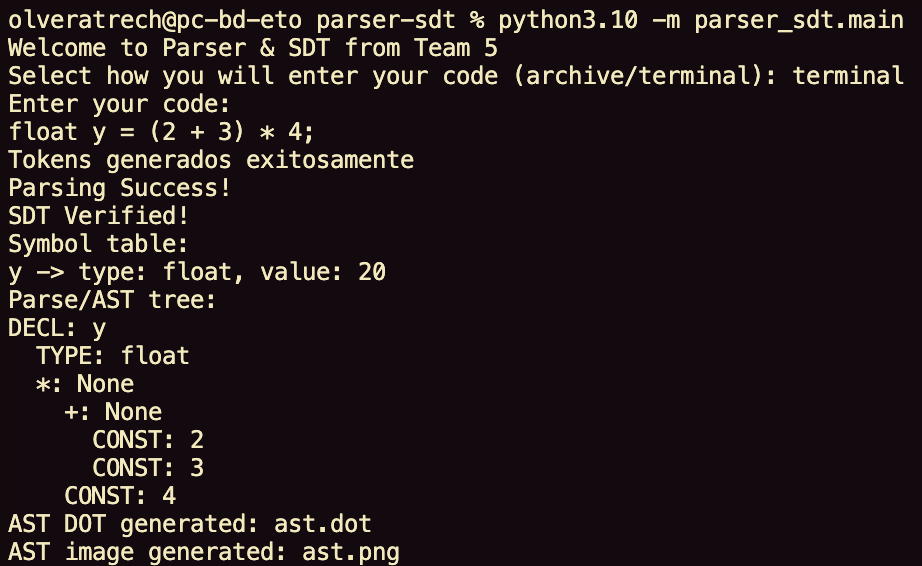
\includegraphics[width=\textwidth]{figs/test1_output.png}
		\caption{Output for Test Case 1: valid declaration and simple expression}
		\label{fig:test1}
	\end{minipage}
	\hfill
	\begin{minipage}[b]{0.25\textwidth}
		\centering
		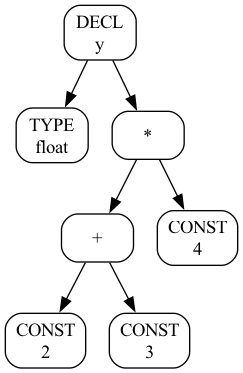
\includegraphics[width=\textwidth]{figs/test1_ast.png}
		\caption{AST for Test Case 1}
		\label{fig:test1_ast}
	\end{minipage}
\end{figure}

\subsubsection{Test Case 2: Valid Declaration with Nested Expressions}

Figure~\ref{fig:test2} shows the output generated for the input \texttt{float y = ((2 + 3) * 4) + (10 * (5 + 1));}. The expression is correctly evaluated to 80, and the AST reflects the nested structure of the operations.

\noindent Figure~\ref{fig:test2_ast} shows the corresponding AST, where the root node is addition (\texttt{+}) with two multiplication subtrees.

\begin{figure}[ht]
	\centering
	\begin{minipage}[b]{0.55\textwidth}
		\centering
		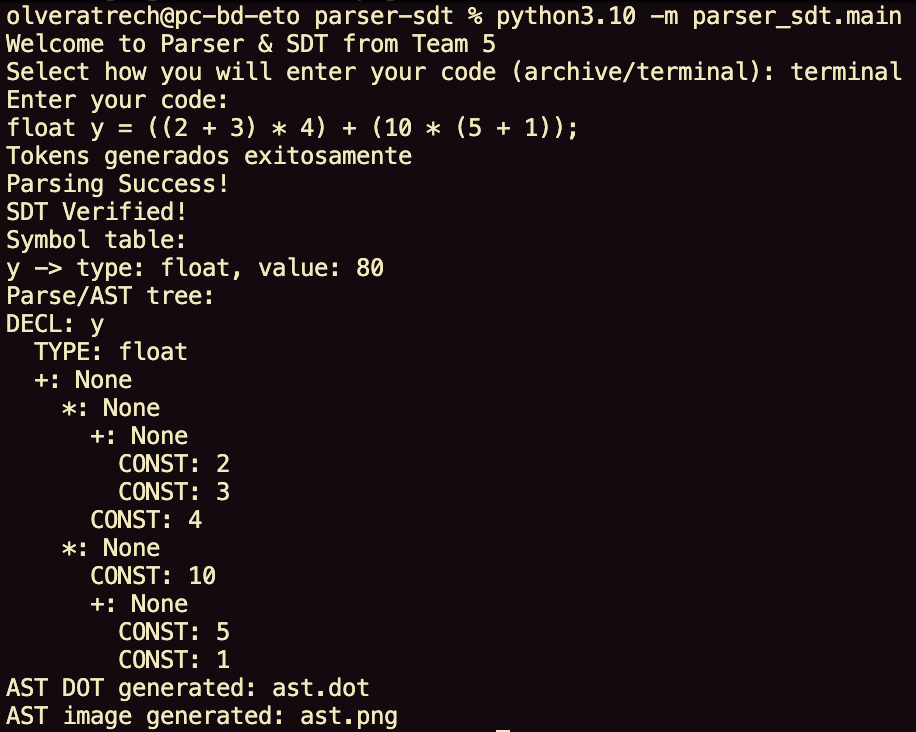
\includegraphics[width=\textwidth]{figs/test2_output.png}
		\caption{Output for Test Case 1: valid declaration and simple expression}
		\label{fig:test2}
	\end{minipage}
	\hfill
	\begin{minipage}[b]{0.4\textwidth}
		\centering
		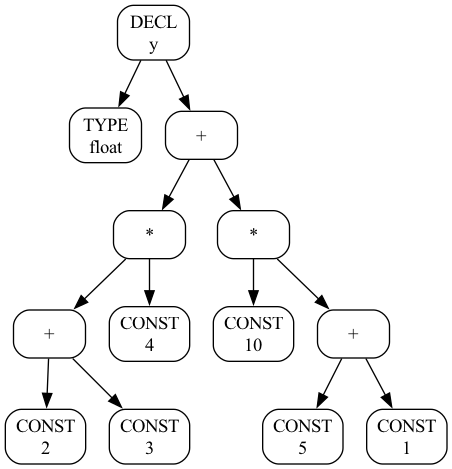
\includegraphics[width=\textwidth]{figs/test2_ast.png}
		\caption{AST for Test Case 1}
		\label{fig:test2_ast}
	\end{minipage}
\end{figure}

\subsection{Invalid Test Cases}

\subsubsection{Test Case 3: Syntax Error - Missing Parenthesis and Semicolon}

For the input \texttt{float y = (2 + 3 * 4}, the system reports a parsing error. The parser cannot complete the reduction because the input does not conform to the grammar.

\begin{figure}[ht]
	\centering
	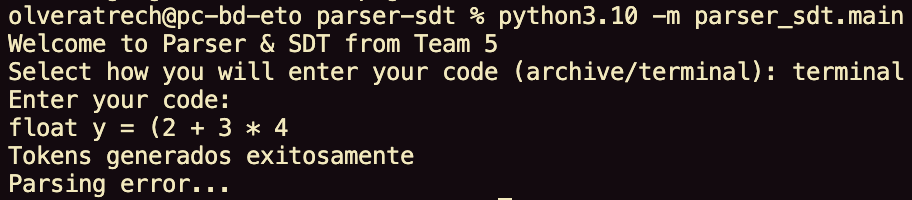
\includegraphics[width=0.6\textwidth]{figs/test3_output.png}
	\caption{Output for Test Case 3: syntax error}
	\label{fig:test3}
\end{figure}

\subsubsection{Test Case 4: Syntax Error - Assignment Without TYPE Keyword}

For the input \texttt{x = 10;}, the system also reports a parsing error. Since the grammar requires a \texttt{TYPE} keyword at the beginning of every statement, this input is syntactically invalid.

\begin{figure}[ht]
	\centering
	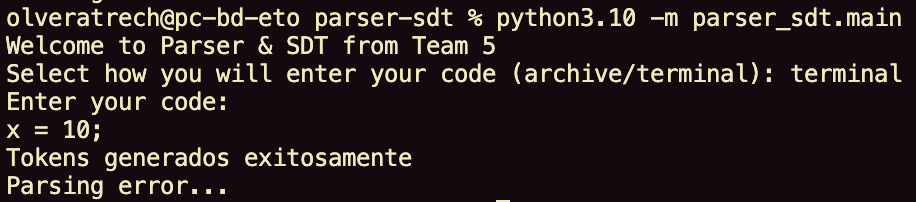
\includegraphics[width=0.6\textwidth]{figs/test4_output.png}
	\caption{Output for Test Case 4: assignment without TYPE keyword}
	\label{fig:test4}
\end{figure}

\subsubsection{Test Case 5: Semantic Error - Type Mismatch}

For the input \texttt{int a = 3.14;}, the parsing succeeds but the SDT fails because an integer variable cannot be initialized with a floating-point constant.

\begin{figure}[ht]
	\centering
	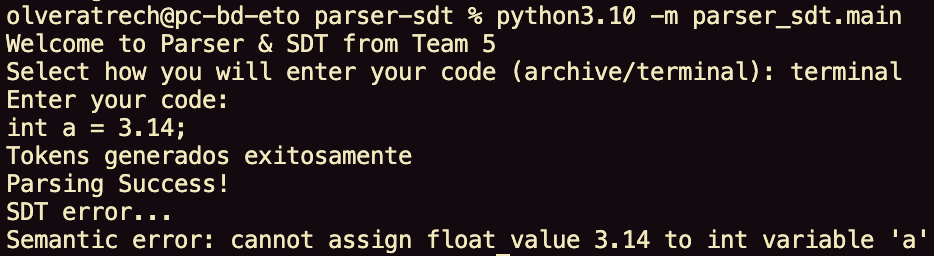
\includegraphics[width=0.6\textwidth]{figs/test5_output.png}
	\caption{Output for Test Case 5: type mismatch}
	\label{fig:test5}
\end{figure}

\subsubsection{Test Case 6: Semantic Error - Variable Used Before Declaration}

For the input \texttt{int x = y + 10;}, the parsing succeeds but the SDT fails because the variable \texttt{y} has not been declared in the symbol table.

\begin{figure}[ht]
	\centering
	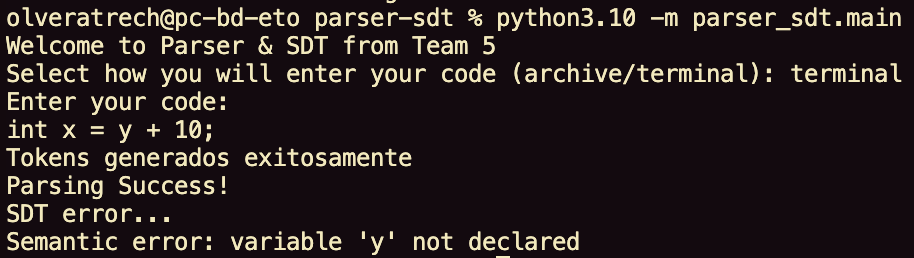
\includegraphics[width=0.6\textwidth]{figs/test6_output.png}
	\caption{Output for Test Case 6: variable used before declaration}
	\label{fig:test6}
\end{figure}

\subsection{Summary of Results}

Table~\ref{tab:summary} presents a consolidated summary of all test cases, indicating whether parsing succeeded, whether SDT verification passed, and the final output message.

\begin{table}[ht]
	\centering
	\footnotesize
	\begin{tabular}{|l|l|l|l|}
		\hline
		\textbf{Test Case} & \textbf{Parsing} & \textbf{SDT} & \textbf{Output} \\
		\hline
		Valid declaration and simple expression & Success & Verified & \texttt{Parsing Success! SDT Verified!} \\
		Valid declaration with nested expressions & Success & Verified & \texttt{Parsing Success! SDT Verified!} \\
		Missing parenthesis and semicolon & Error & — & \texttt{Parsing error...} \\
		Assignment without TYPE keyword & Error & — & \texttt{Parsing error...} \\
		Type mismatch (int = float) & Success & Error & \texttt{Parsing Success! SDT error...} \\
		Variable used before declaration & Success & Error & \texttt{Parsing Success! SDT error...} \\
		\hline
	\end{tabular}
	\caption{Summary of test results}
	\label{tab:summary}
\end{table}
\newpage

\section{Conclusions}

The development of this syntax and semantic analyzer demonstrates the successful application of theoretical compiler concepts to a functional implementation. The results presented in Section 4 show that the LALR parser correctly validates the syntactic structure of the input language according to the defined context-free grammar, while the SDT effectively enforces semantic rules and builds auxiliary structures such as the symbol table and the abstract syntax tree.

The implementation confirms that bottom-up parsing using an LALR(1) table, constructed from first principles via closure, goto, and state merging, is a viable approach for languages with deterministic context-free grammars. The shift-reduce algorithm, combined with two stacks (states and semantic values), faithfully simulates the LR automaton and provides a natural integration point for syntax-directed translation.

The distinction between parsing errors and semantic errors, as shown in the test cases, validates the modular separation of concerns within the compiler pipeline. Syntactic errors are detected and reported by the parser before any semantic action is executed, while inputs that are syntactically correct but violate semantic rules (type mismatches, undeclared variables, use before initialization) are properly caught by the SDT during reduction actions. This separation is essential for building robust compilers that provide meaningful feedback to the user.

The construction of the AST and the symbol table during the parsing process demonstrates how context-sensitive information can be embedded into a context-free grammar framework. The AST abstracts away irrelevant syntactic details (parentheses, semicolons) while preserving the hierarchical structure of operations, which is a necessary step for subsequent phases such as intermediate code generation and optimization.

In summary, the theoretical concepts covered in class—LR items, closure, goto, FIRST sets, LALR table construction, shift-reduce parsing, and syntax-directed translation—were directly applied to build a working analyzer. The system meets all the specified requirements: it reads tokens from a lexical analyzer, validates syntax according to a CFG, executes SDT rules, and produces a symbol table and an AST. The results confirm that a bottom-up LALR parser with integrated semantic actions can be implemented from scratch without relying on parser generators, providing a deep understanding of how compilers verify program correctness at both the syntactic and semantic levels.

\printbibliography
\end{document}